\chapter{M\'ethodologie}
\label{ChapMethodologie}

	\section{Les m\'ethodologies de d\'eveloppement web \cite{MethodologieDeDeB,MethodologieDeDeA,MethodologieDeDeC}}

		\paragraph{}Une m\'ethodologie de d\'eveloppement logiciel est un ensemble de techniques, de principes et de m\'ethodes qui guident le processus de d\'eveloppement afin de garantir la r\'eussite du d\'eveloppement. Il existe plusieurs m\'ethodologies de d\'eveloppement logiciel dont:  Agile, Waterfall, DevOps, Rapid Application Development (RAD), Scaled Agile Framework (SAFe), etc. Chacun pr\'esente \`a la fois des avantages et des inconv\'enients en sorte que le choix d'une m\'ethodologie d\'epende de plusieurs param\`etres tels que: Les conditions de travail, les objectifs \`a atteindre, les connaissances des membres du groupe, entre autres.

			\subsection{La m\'ethode Agile}
				\textit{La m\'ethode agile est une m\'ethodologie de gestion de projet ouverte au changement. Elle s'oppose aux m\'ethodologies de gestion de projet traditionnelles qui s'organisent selon un mode de travail s\'equentiel.\\
				La m\'ethode agile est organis\'ee en cycles de d\'eveloppements courts. Le produit final est d\'evelopp\'e au fur et \`a mesure.\\
				L'\'equipe agile est invit\'ee \`a collecter du feedback le plus t\^ot possible aupr\`es des utilisateurs du produit, afin de prendre en compte leurs remarques dans le prochain cycle de d\'eveloppement. Le produit est ainsi construit de fa\c{c}on collaborative.}\cite{MethodeAgile}.

			\subsection{La m\'ethode Waterfall}
				\textit{La m\'ethodologie Waterfall est une approche traditionnelle du d\'eveloppement d'applications web. Il s'agit d'un processus lin\'eaire, o\`u chaque \'etape du processus de d\'eveloppement suit l'\'etape pr\'ec\'edente}\cite{MethodologieDeDeB}. Elle est relativement simple \`a mettre en œuvre et \`a comprendre mais elle peut \^etre longue \`a mettre en \oe{}uvre et est peut flexible.

			\subsection{M\'ethodes hybrides}
				Il est possible d'utiliser des \'el\'ements de plusieurs m\'ethodologies dans un m\^eme projet. Dans ce cas, la m\'ethodologie utilis\'ee est dite \textit{une m\'ethodologie hybride}.


	\section{Les frameworks}
		\textit{Un framework est une infrastructure conceptuelle qui fournit une structure g\'en\'erale pour un domaine particulier. Il s'agit grosso-modo d'un ensemble de principes \`a respecter dans l'organisation d'un projet. Un framework offre des lignes directrices et des recommandations g\'en\'erales pour aborder les probl\`ames complexes de gestion de projet.}\cite{Framework} Il en existe de nombreux, qui concernent le d\'eveloppement de logiciel dont Scrum, Kanban et bien d'autres.

		\subsection{Scrum\cite{Scrum}}
			Le framework Scrum repose sur l'apprentissage continu et l'adaptation \`a des facteurs variables. Il reconna\^it qu'au d\'emarrage d'un projet, l'\'equipe ne sait pas tout, et qu'il \'evoluera avec l'exp\'erience. Scrum est structur\'ee pour aider les \'equipes \`a s'adapter naturellement \`a l'\'evolution des conditions et des exigences des utilisateurs. La red\'efinition des priorit\'es et les cycles de livraison courts sont int\'egr\'es au processus. Mais, m\^eme s'il est structur\'e, il n'est pas rigide et peut \^etre adapt\'ee aux besoins. Scrum encourage l'\'equipe \`a apprendre par l'exp\'erience, \`a s'auto-organiser pendant qu'elle tente de r\'esoudre un probl\`eme.

\begin{figure}[ht]
	\centering
	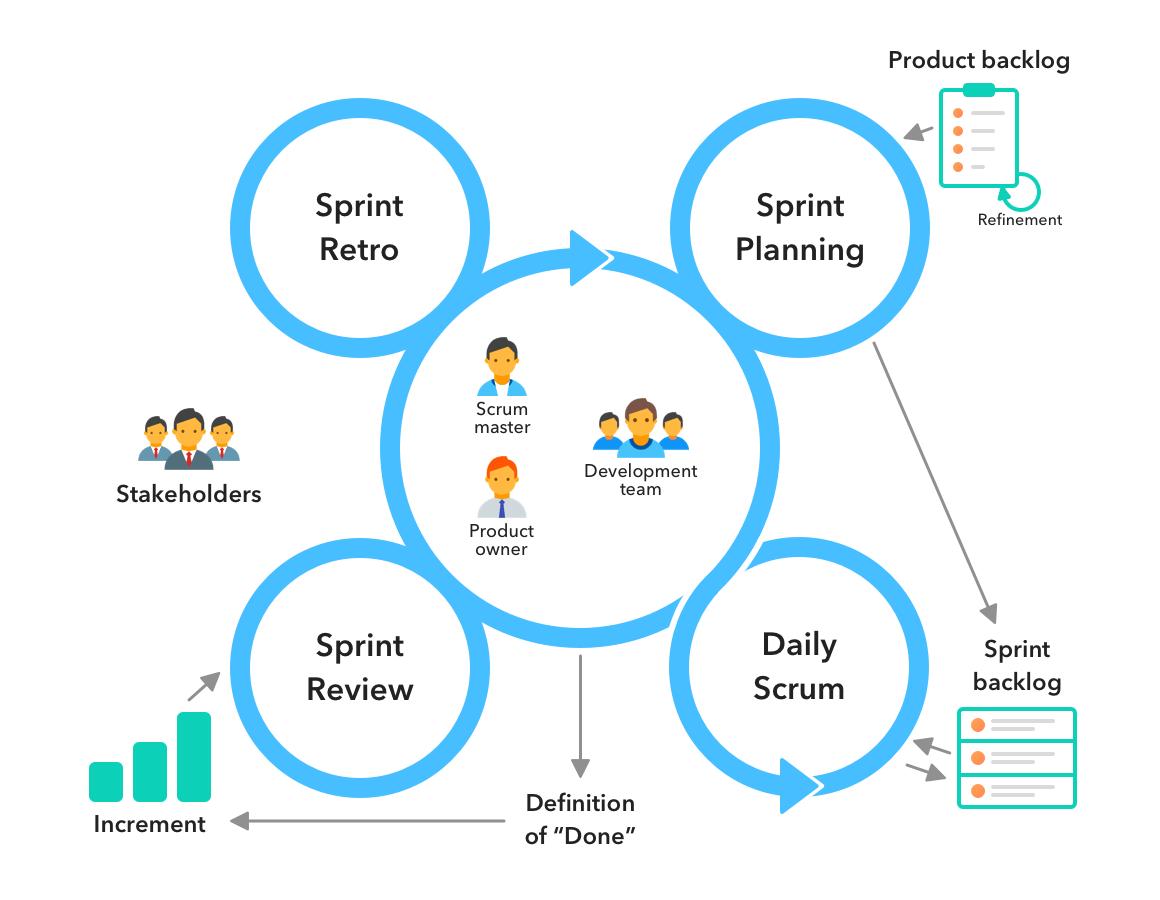
\includegraphics[width=0.75\linewidth]{Pictures/Scrum.jpeg}
	\caption{Framework Scrum \textbf{Source} \href{https://startinfinity.com/project-management-methodologies/scrum}{startinfinity.com})}
	\label{scrum}
\end{figure}


	\section{M\'ethodologies et frameworks choisis}
		Pour choisir la m\'ethodologie \`a adopter dans la r\'ealisation de notre projet, nous nous proposons d'en trouver une qui soit r\'ealisable dans notre environnement de travail. Consid\'erant ce dernier comme \'etant le param\`etre le plus contraignant dans notre cas. Ensuite nous d\'esirons qu'elle favorise la communication entre les diff\'erentes acteurs et qu'elle soit efficace.

		\paragraph{} Pour notre part, nous travaillons dans le contexte que d\'ecrivent les points suivants:
			\begin{itemize}
				\item[-] Nous habitons respectivement Mariani, Route Fr\`eres et Delmas.
				\item[-] Pour nous rencontrer en ville, deux d'entre nous doivent traverser des zones de non droit
				\item[-] La couverture r\'eseau \`a ces trois endroits n'est ni stable, ni similaire. Il peut donc arriver que l'un d'entre nous ne soit pas joignable via Whatsapp, Telegram ou appel t\'el\'ephonique \`a cause d'une panne de r\'eseau.
				\item[-] L'activit\'e des gangs arm\'es peut emp\^echer les d\'eplacement de n'importe lequel d'entre nous, \`a n'importe quel moment.
				\item[-] Au moment o\`u nous d\'emarrons le projet, nous ne disposons pas de toutes les connaissances n\'ecessaires pour sa r\'ealisation.
			\end{itemize}


		\paragraph{}Au d\'ebut, pour fonder les bases de notre collaboration avec le client, la m\'ethode utilis\'ee \'etait la m\'ethode Watherfall. Ensuite nous avons pris les d\'ecisions suivantes:
		\begin{enumerate}
			\item Pour des raisons de s\'ecurit\'e, nous devons limiter les rencontres en pr\'esentiel.

			\item Compte tenu de notre choix pour l'architecture du syst\`eme (voir chapitre~\ref{ChapArchitectureDuSysteme}), nous avons donc divis\'e le travail en cinq grandes parties autonomes, mais co-d\'ependantes:
				\begin{enumerate}
					\item R\'edaction du document de m\'emoire
					\item D\'eveloppement de l'interface utilisateur
					\item D\'eveloppement de l'application cot\'e serveur
					\item D\'eveloppement de la base de donn\'ees.
					\item D\'eploiement du site
				\end{enumerate}

			\item Chacun de nous est responsable de tout ce qui concerne le projet dans son ensemble maus se charge d'une ou d'au moins une partie en priorit\'e. Permettant \`a chacun de continuer \`a travailler m\^eme s'il se retrouve provisoirement isol\'e de l'\'equipe.
		\end{enumerate}






	 	\paragraph{} Compte tenu de nos objectifs, de notre contexte et environnement de travail et de nos contraintes nous utilisons la m\'ethode \textbf{Agile} \`a travers son Framework \textbf{Scrum} pour d\'eterminer des cycles de travail \`a court terme ensuite, suivant le contexte environnemental, nous utiliseront soit Scrum soit Waterfall pendant ces cycles.
	